%%%%%%%%%%%%%%%%%%%%%%%%%%%%%%%%%%%%%%%%%%%%%%%%%%%%%%%%%%%%%%%%%%%%%%%%%%%%%%%%%%%%%%%%
\clearpage
\section{Form factors of magnetic objects} \hspace{1pt}
\label{sec:magneticstructures}

\subsection{Magnetic spin misalignment} \hspace{1pt}
\label{sec:spinmisalignment}

In \cite{Michels2013} the autocorrelation function $C(r)$ of the
spin misalignment has been published. The approach assumes the
material to be close to magnetic saturation and considers uniform
values for the exchange interaction and the saturation
magnetization, i.e. it's a micro magnetic theory of single phase
magnets. The correlation function is defined by
\begin{align}
C(r) & = \frac{K R^4}{H_i^2} \int_0^\infty
\frac{j_0(qr)j_1^2(qR)}{\left(1+l_H^2q^2\right)^2} d\text{q}
\end{align}
where $j_1$ and $j_2$ are the spherical Bessel
functions\footnote{the spherical Bessel functions $j_n$ and $y_n$,
and are related to the ordinary Bessel functions $J_n$ and $Y_n$ by:
 $j_{n}(x) = \sqrt{\frac{\pi}{2x}} J_{n+\frac{1}{2}}(x)$ and $
 y_{n}(x) = \sqrt{\frac{\pi}{2x}} Y_{n+\frac{1}{2}}(x) = (-1)^{n+1}
 \sqrt{\frac{\pi}{2x}}J_{-n-\frac{1}{2}}(x)$.
 The first two spherical Bessel function are computed by
 $j_0(x)=\frac{\sin(x)} {x}$ and
 $j_1(x)=\frac{\sin(x)} {x^2}- \frac{\cos(x)} {x}$} and $K=8H_P^2/V$.
 $H_i$ is the internal magnetic field, $l_H=\sqrt{2A/(\mu_0 M_s H_i)}$
 the exchange length of the magnetic field, $H_P$ the mean magnetic
 anisotropy field, $A$ the exchange-stiffness constant, and $\mu_0$
 the permeability of free space. The internal magnetic field
 $H_i=H_0-NM_s$ is the sum of the external applied magnetic field
 $H_0$ and the demagnetisation field $-NM_s$ ($N$: demagnetisation
 factor). $V$ is the sample volume and $M_s$ the saturation
 magnetisation.

It is assumed in this model that the magnetic anisotropy field,
which perturbs the magnetization from the homogeneously magnetized
state, is uniform (constant) within a spherical volume; the
parameter $R$ represents the corresponding "anisotropy-field"
radius, and it is emphasized that $R$ is not necessarily identical
to the crystallite size.

The correlation is related to the scattering intensity by
\begin{align}
C(r) &= \frac{1}{2\pi^2} \int_0^\infty I(q) q^2
\frac{\sin(qr)}{qr}d\text{q}
 = \frac{1}{2\pi^2} \int_0^\infty I(q) q^2 j_0(qr) d\text{q}
\end{align}
Therefore the intensity $I(q)$ can be
computed as
\begin{align}
I(q) & = \frac{K R^6}{H_i^2}
\frac{2\pi^2}{\left(qR\right)^2}\frac{j_1^2(qR)}{\left(1+l_H^2q^2\right)^2}
\end{align}

\vspace{5mm}

\hspace{1pt}\\
\uline{Input Parameters for the models \texttt{C(r) for spin
misalignment} and} \newline \uline{\texttt{I(q) for spin misalignment}:}\\
\begin{description}
\item[\texttt{K}] $K=8H^2_P/V$
\item[\texttt{H\_i}] internal magnetic field $H_i$
\item[\texttt{l\_H}] exchange length of magnetic field $l_H$
\item[\texttt{R}] anisotropy field radius $R$
\end{description}

\noindent\uline{Note:}
none


\begin{figure}[htb]

\begin{subfigure}[b]{0.48\textwidth}
   \centering
   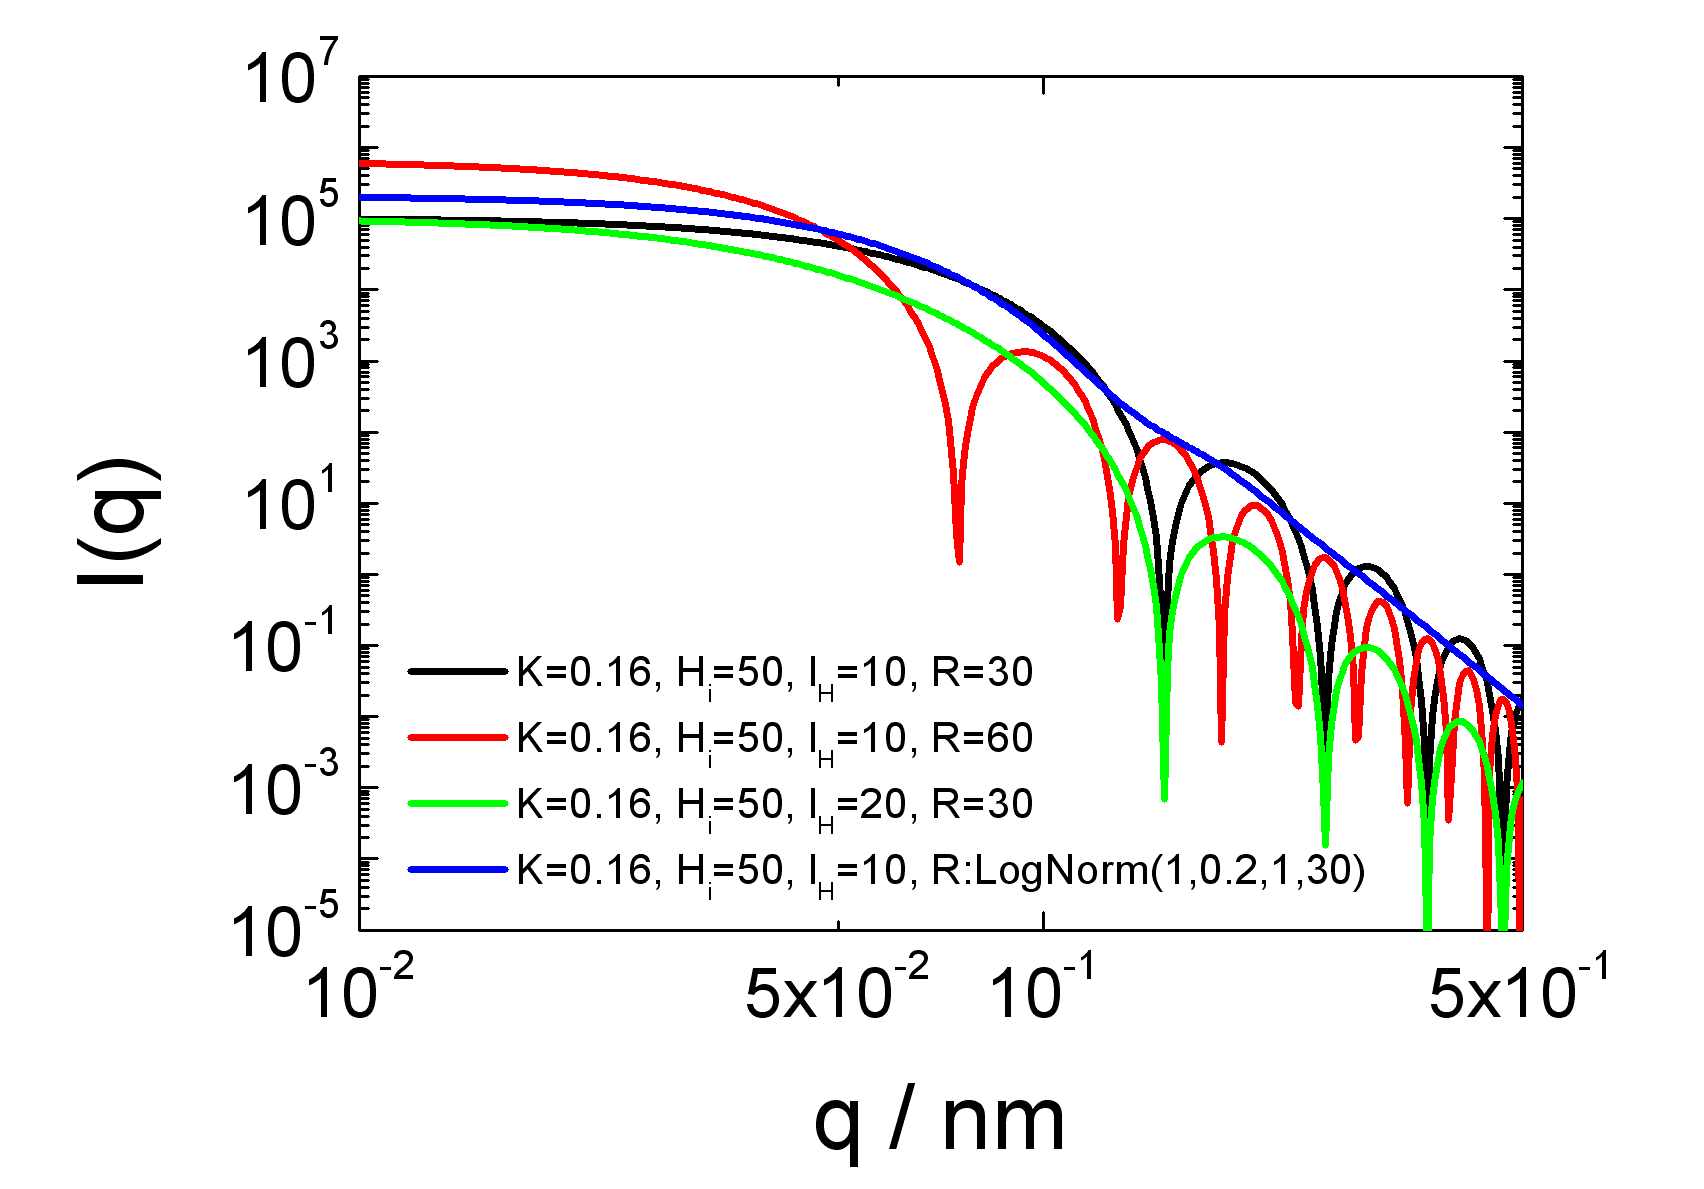
\includegraphics[width=\textwidth]{../images/form_factor/magnetic/IQ4spinmisalignment.png}
   \caption{The scattering curves for the correlation functions to the right}
   \label{fig:MagSpinMisAlignment1}
\end{subfigure}
\hfill
\begin{subfigure}[b]{0.48\textwidth}
   \centering
   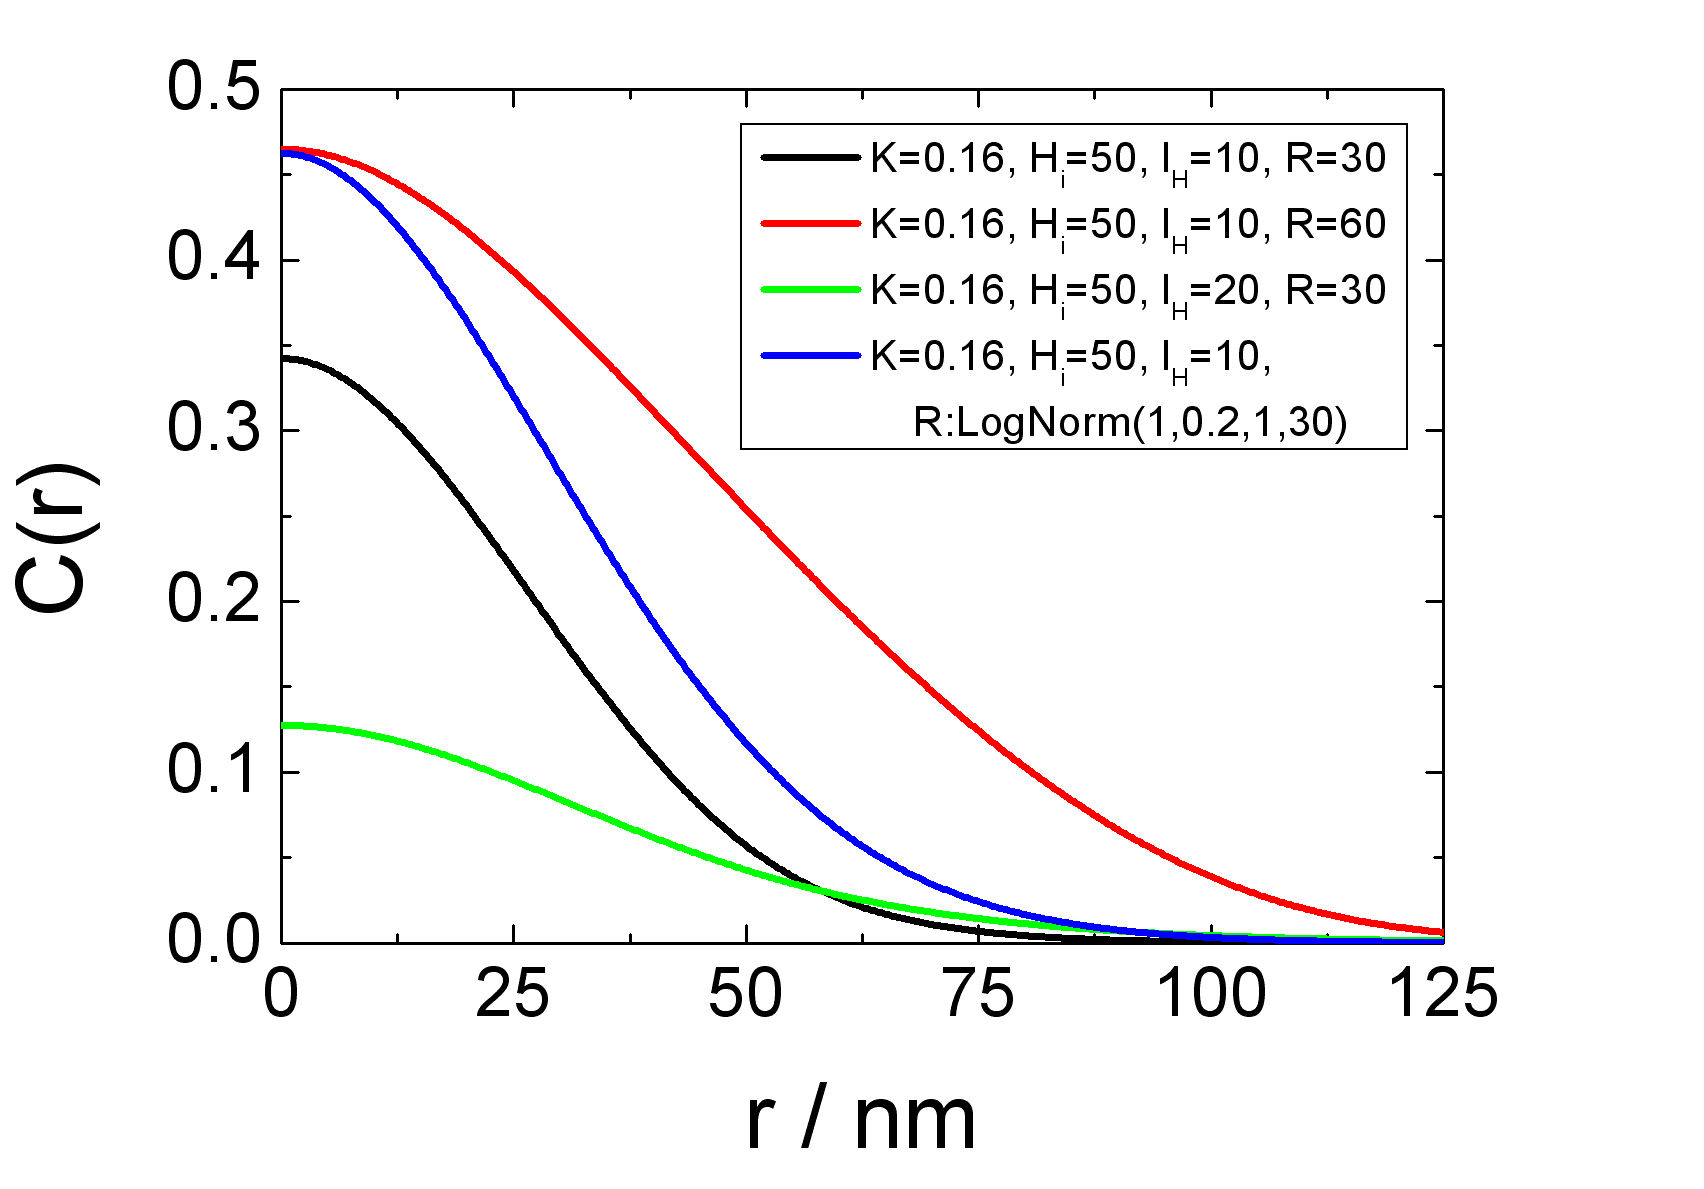
\includegraphics[width=\textwidth]{../images/form_factor/magnetic/correlation4spinmisalignment.png}
   \caption{correlation functions for the scattering curves to the left}
   \label{fig:MagSpinMisAlignment2}
\end{subfigure}
\caption{Scattering curves and corresponding correlation functions.
In one case the radius of the anisotropy field is assumed to have a
lognormal size distribution.} \label{fig:MagSpinMisAlignment}
\end{figure}


%%%%%%%%%%%%%%%%%%%%%%%%%%%%%%%%%%%%%%%%%%%%%%%%%%%%%%%%%%%%%%%%%%%%%%%%%%%%%%%%%%%%%%%%
\clearpage
\subsection{Ferrofluids} \hspace{1pt}
\label{sec:ferrofluid}

"Ferrofluids" and "Magnetic Liquids" are two common expressions for
suspensions in which nanometer sized particles are dispersed in a
carrier liquid. Figure \ref{fig:ferrofluidparticle} gives a
schematic illustration. The particle material can be ferri- or
ferromagnetic, and is often coated with a stabilizing dispersing
agent (surfactant). The particle size is smaller than the size of
magnetic domains of the corresponding bulk material. This means that
every particle is single-domain ferri- or ferromagnetic.
Additionally we assume in this model, that the metallic core has a
shell structure to be able to model a thin oxidation layer with a
reduced magnetisation on the surface.The surfactant molecules
consist of a head and a polar tail. The head can coalesce with the
magnetic particle, and the tail protrudes into the carrier liquid
and can dissolve in it. This polar tails protruding into the liquid
lead to repulsion between the colloids. Different substances like
organic acids or polymers usually serve as surfactants. The carrier
liquid is selected to meet the requirements for a particular
applications: It can be hydrocarbon, ester, water or others. As a
result of the small size of the particles they are very mobile due
to Brownian motion. In zero field the magnetic moment is random
oriented. Applying a magnetic field the orientation distribution of
the magnetic moments of the ferrofluid particles follow a Langevin
statistic.

\begin{figure}[htb]
\begin{center}
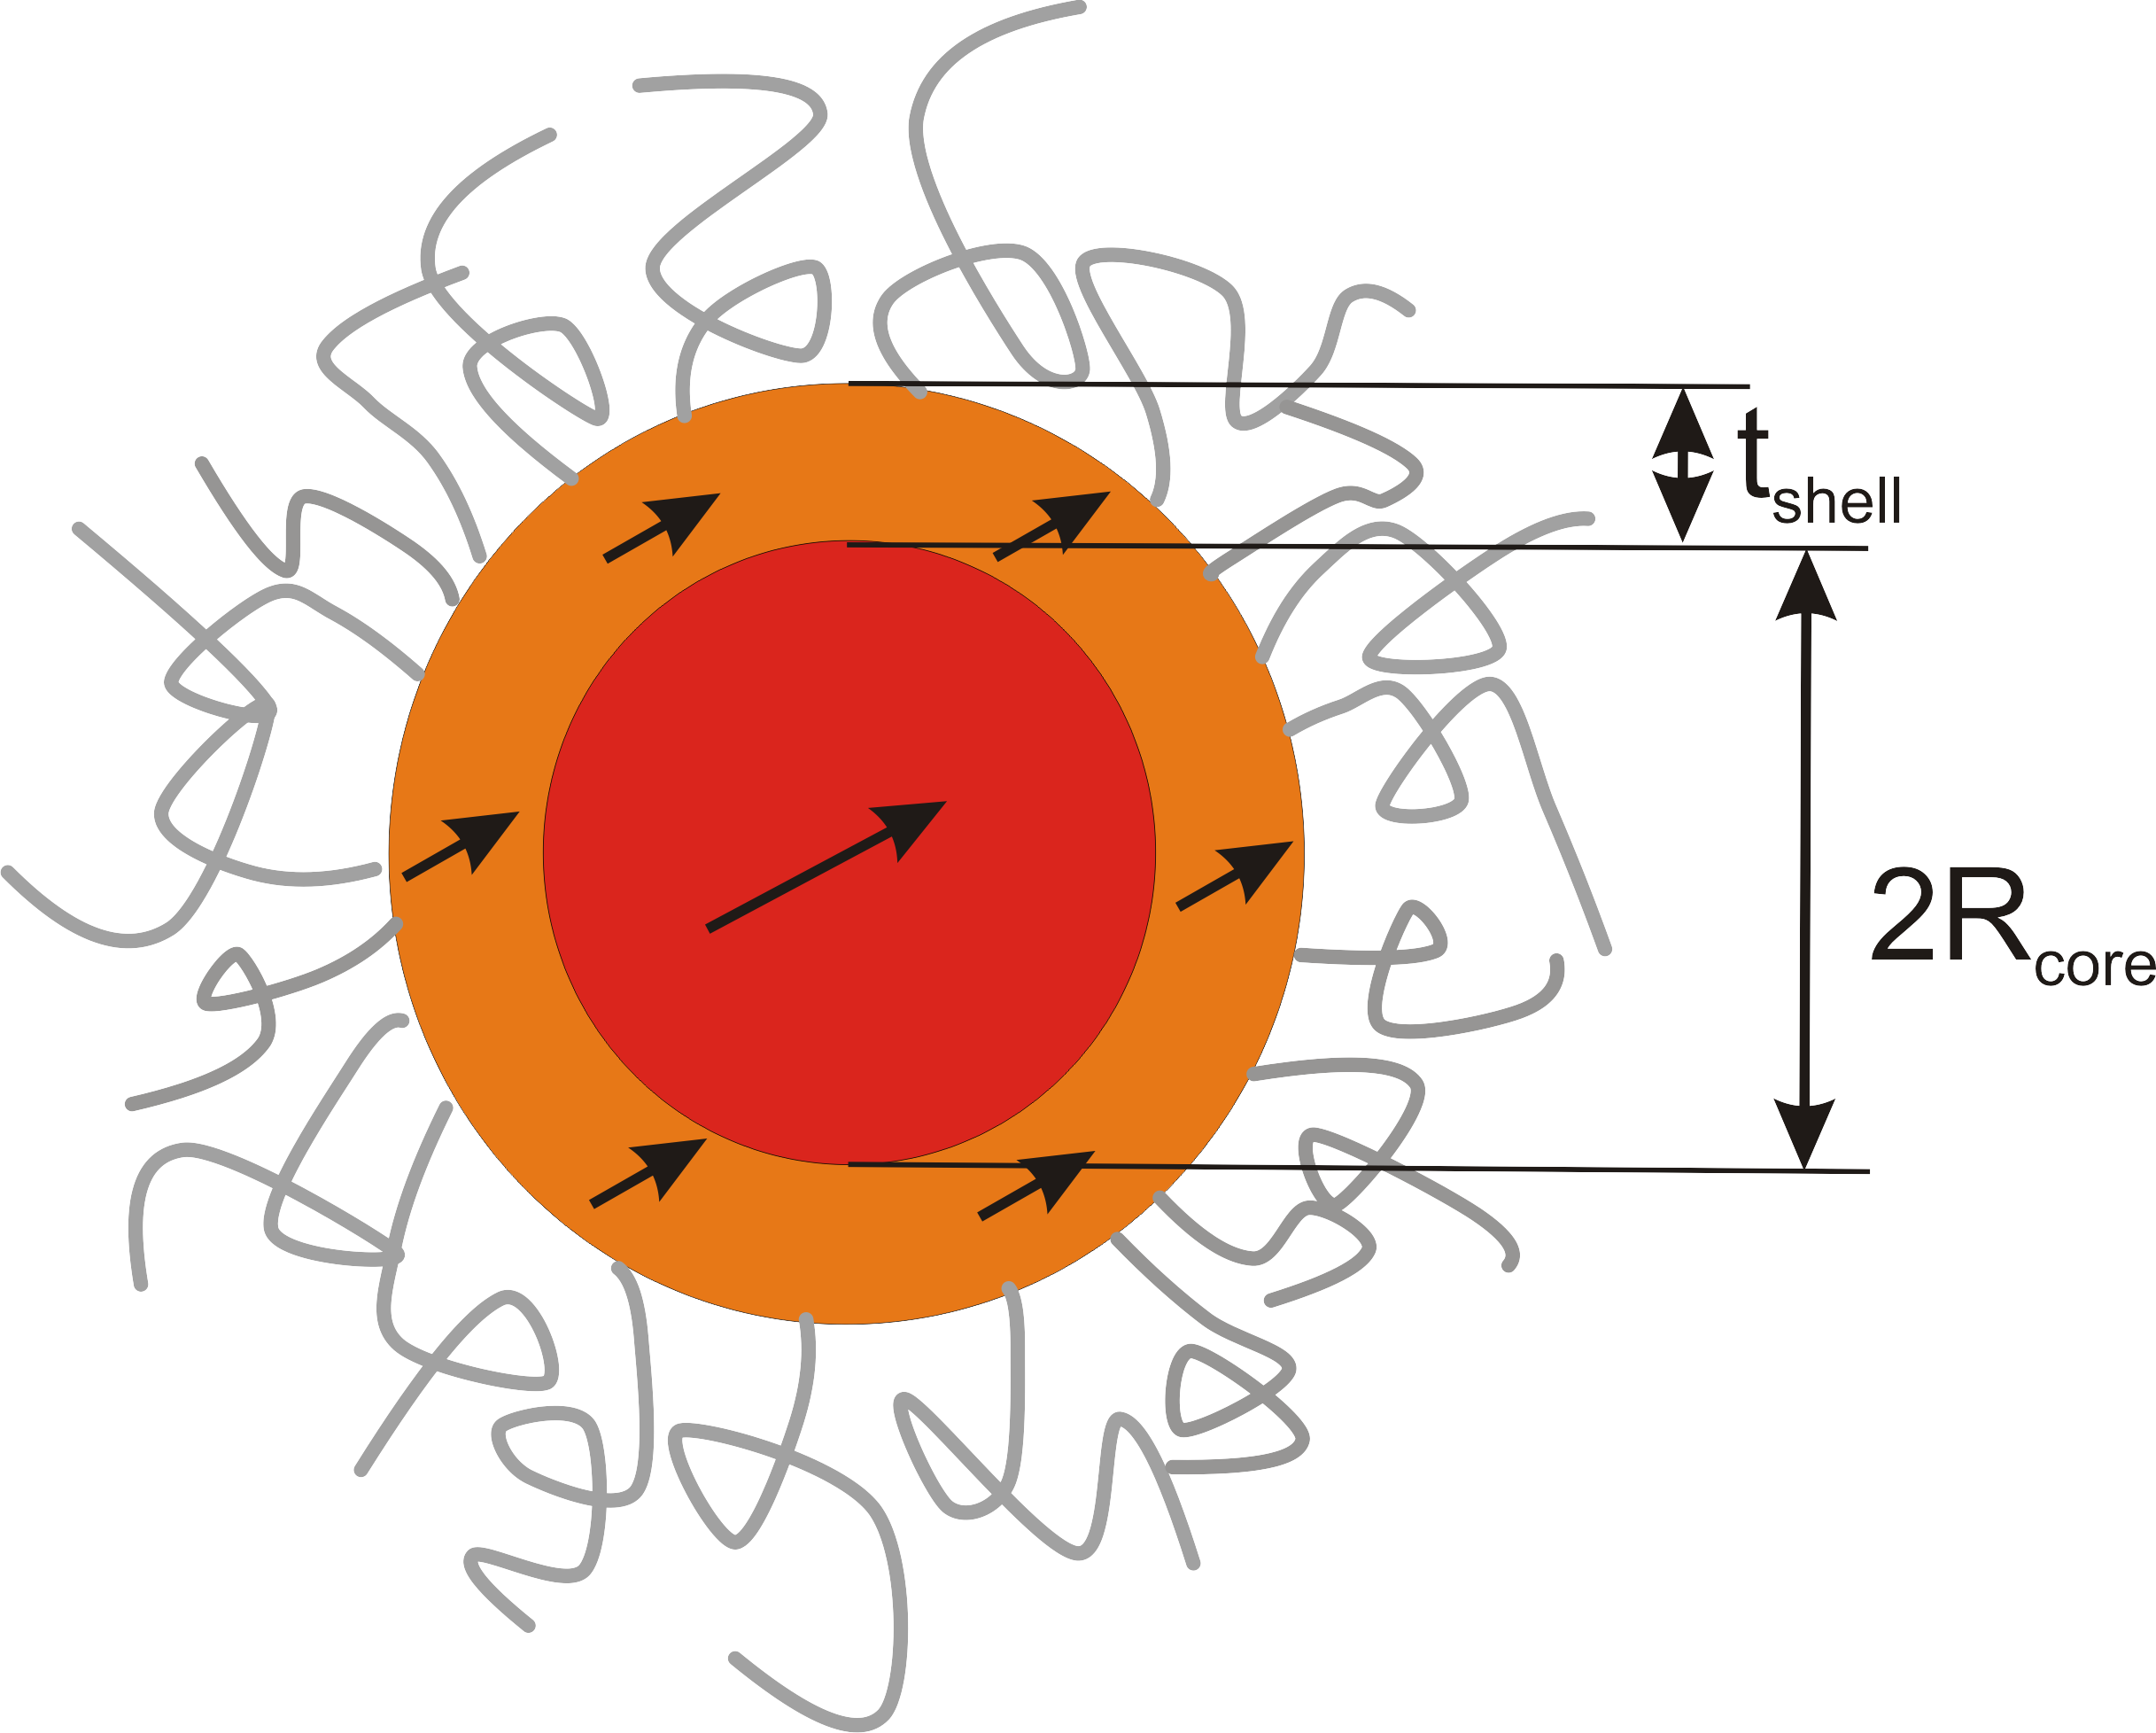
\includegraphics[width=0.6\textwidth]{../images/form_factor/ferrofluid/ferrfluidparticle.png}
\end{center}
\caption{Sketch of a ferrofluid particle stabilised with surfactant
molecules on its surface. The magnetic core can have a shell with
lower magnetisation. The direction of the shell magnetisation is
assumed to be parallel or antiparallel to the core magnetisation,
depending on the signs of the magnetic scattering length densities.}
\label{fig:ferrofluidparticle}
\end{figure}

In the present implementation of scattering function of
superparamagnetic particles geometrical parameters are calculated
like magnetic scattering length densities are calculated from the
magnetization of the shell and the core, whereas the nuclear
scattering length densities are an explicit input parameter. In such
a case one has to be careful using the right units.

The relevant parameters to describe the ferrofluid particle in this
model are:
\begin{itemize}
\item Radius of the $R_\text{core}$ in reciprocal units of scattering vector $q$.
\item Thickness of the metallic shell $t_\text{shell}$ in reciprocal units of scattering vector $q$.
\item Specific aggregation number of stabilizing surfactant molecules per surface area in units of cm$^{-2}$.
\item Molecular volume $V_\text{brush}$ of a single surfactant molecule in units of nm$^3$.
The scattering length density calculator of \SASfit might be useful
to supply this value.
\item Nuclear scattering length density $\eta_\text{core}$ of the solid ferromagnetic core.
\item Nuclear scattering length density $\eta_\text{sh}$ of an optional demagnetised shell of the
solid ferromagnetic core.
\item Nuclear scattering length density of the solvent $\eta_\text{solv}$.
\item Magnetisation of the metallic core $M_\text{core}$.
      The magnetic scattering length density is calculated via eq.\ \ref{eq:magnetic_SLD}.
\item Magnetisation of the metallic shell $M_\text{sh}$.
      Also here the magnetic scattering length density of the shell is calculated via eq.\ \ref{eq:magnetic_SLD}.
\item Temperature $T$ in Kelvin.
\item External applied magnetic field $B$ in Tesla or milliTesla depending of the units of $q$.
\item Lagrange parameter $\alpha$ for describing superparamagnetic properties is calculated by ratio
of the potential energy of the total magnetic moment of the superparamagnetic particle in the applied magnetic
field to the thermal energy via eq.\ \ref{eq:alpha}
\item As aligned magnetic structures scatter anisotropically the angle $\psi$ between scattering vector
and the applied magnetic field needs to be supplied.
\item using polarised neutrons the incident polarisation $p$ needs to be known. $p$ can have values $p \in [-1,1]$.
\item in case of full polarisation analysis also the transmission of the analyser needs to be known
\end{itemize}

The magnetic scattering length density $\eta_\text{mag}$ in units of
cm$^{-2}$ is calculated from the magnetisation $M$ given in units of
A/m by
\begin{align}
\eta_\text{mag} &= D_M \mu_0 M \label{eq:magnetic_SLD} \times 10^{-4}\\
D_M & = 2.3161 \frac{1}{\text{Vs}} \\
\mu_0 &= 4\pi \times 10^{-7} \text{H}\text{m}^{-1} = 4\pi \times 10^{-7} \frac{\text{Vs}}{\text{Am}}
\end{align}
To get the magnetic scattering length density in cm$^{-2}$ a
multiplication factor of $10^{-4}$ has to be applied. By choosing
the unit cm$^{-2}$ for the magnetic scattering length density we
have to use the corresponding units for the nuclear scattering
length densities.

The other unit which has to be chosen with care is the molecular
volume $V_\text{brush}$ of a single surfactant molecule. From the
specific aggregation and the molecular volume the excess scattering
of the surfactant shell is calculated. In case that the $q$-values
are given in units of nm$^{-1}$ the molecular volume has to be in
units of  nm$^3$ and in case of \AA$^{-1}$ for the q-values one also
need to use \AA$^{3}$ units for the molecular volume.

The next parameter, where we need to use proper units is the
Langevin parameter $\alpha$, describing the ratio between potential
energy of the magnetic moment of the particle to the thermal energy:
\begin{align}
\alpha &= \mu_\text{FF}B/(k_B T) \label{eq:alpha} \\
\mu_\text{FF} &= \frac{4}{3}\pi
\left[ R_\text{core}^3  M_\text{core} +
\left\{\left(R_\text{core}+t_\text{shell}\right)^3-R_\text{core}^3\right\} M_\text{shell}
\right] \times \frac{10^{-27}\text{m}^3}{\text{nm}^3}\label{eq:mu_FF}\\
k_\text{B} &= 1.3806488 \times 10^{-23} \text{m}^2 \text{kg} \text{
s}^{-2} \text{K}^{-1}
\end{align}
The magnetic moment of a particle $\mu_\text{FF}$ as given in eq.\
\ref{eq:mu_FF} is calculated from the magnetisation of the core and
the shell and their corresponding dimensions. The magnetisation has
units of A/m whereas the radius and shell thickness have reciprocal
dimensions of $q$. A magnetic moment is measured in ampere–square
meters (Am$^2$) or in joules per tesla (JT$^{-1}$) which is
equivalent: $1 \mathrm{Am}^2 = 1 \mathrm{JT}^{-1}$. In case that $q$
values are given in \AA$^{-1}$ the applied magnetic field should be
given in units of mT instead of T.

The implemented form factor for ferrofluids is done for neutrons
with or without incident polarisation as well as with polarisation
analysis. In case of full polarisation analysis the measured
intensity $I_m(\mathbf{Q})$ would depend on the incident
polarisation, efficiency of the spin-flipper and in case of an
opaque spin filter from its transmission values for the two spin
states according to eq.\ \ref{eq:Im(Q)_POLARIS}. However here we
just have implemented the intensities for a given incident
polarisation without polarisation analysis (SANSPOL) and the
intensities for POLARIS data are assumed to be corrected so that the
resulting intensities correspond to perfect incident polarisation
and perfect polarisation analysis. For calculating the scattering
cross-section for the 4 scattering processes involved the
differential cross-sections in the decoupling approach are given by
\begin{align} \label{eq:dsigma_dOmega_ijSQ}
\frac{\mathrm{d}\sigma_{{\pm\pm}\atop{\pm\mp}}}{\mathrm{d}\Omega}(\BM{Q})
&= N\left\{ \left\langle
\abs{F_{{\pm\pm}\atop{\pm\mp}}(\BM{Q})}^2\right\rangle +
\abs{\left\langle F_{{\pm\pm}\atop{\pm\mp}}(\BM{Q})\right\rangle}^2
(S(\BM{Q})-1) \right\}
\end{align}
The averages $\langle\rangle$ needs to be performed over the
orientation distribution of the superparamagnetic moments of the
ferrofluids and later on also about their size distribution. The
averaging over the orientation distribution of the magnetic moments
can be done analytically in terms of order parameters according to
\cite{Wiedenmann2011,Wagner2005,Kohlbrecher1997}.

The spin dependent scattering amplitudes
$F_{{\pm\pm}\atop{\pm\mp}}(\BM{Q})$ can be calculated from the
nuclear and magnetic amplitudes
\begin{align}
F_{\pm\pm}(\BM{Q}) & = F_N(\BM{Q}) \mp F_{M_\perp x}(\BM{Q}) \\
F_{\pm\mp}(\BM{Q}) & = -\left(F_{M_\perp y}(\BM{Q}) \pm \imath
F_{M_\perp z}(\BM{Q})\right)
\end{align}
The nuclear scattering amplitude is proportional to the nuclear
excess scattering $\beta_N=F_N(Q=0)$ and the nuclear form factor
$f_N(\BM{Q})$
\begin{align}
F_N(\BM{Q}) &= \beta_N f_N(\BM{Q})
\end{align}
The magnetic scattering amplitude $\BM{F}_{M_\perp}(\BM{Q})$ can be
described as a vector, with
\begin{align}
\BM{F}_{M_\perp}(\BM{Q}) =  \BM{\hat{\mu}}_\perp D_M \mu_\text{FF}
f_M(\BM{Q})=\BM{\hat{\mu}}_\perp F_M(\BM{Q})
\end{align}
where $f_M(Q)$ is the magnetic form factor, $\BM{\mu}_\text{FF}$ the
magnetic moment of the particle, $D_M=\frac{\gamma e}{2\pi\hbar}$,
and $\BM{\hat{\mu}}_\perp$ the Halpern-Johnson vector defined as
\begin{align}
\BM{\hat{\mu}}_\perp &=
\frac{\BM{Q}}{Q}\times\left(\frac{\BM{\mu}_\text{FF}}{\mu_\text{FF}}\times\frac{\BM{Q}}{Q}\right)
\end{align}
It is assumed here that the neutron spin polarization is parallel or
antiparallel to the axes $\BM{e}_x$ which is the direction
perpendicular to the incoming neutron beam.

In the following we derive the average over the squared scattering
amplitude and the averaged scattering amplitude for
superparamagnetic particles. The description of the nuclear
scattering amplitude is based on the form factor described in
\cite{PedersenGerstenberg96,PedersenJApplCryst2000} for block
copolymer micelles from Pedersen et al.

The different versions of form factor implemented in the plugin
differ on one side on the model for describing the scattering of the
molecules on the surface and on the other side how the data are
pre-treated. At the moment three different model for the polymer
chains on the surface are implemented, namely that the chains are
noninteracting and follow random walk behaviour \texttt{(Chain,RW)},
secondly they are interacting due to the high grafting density and a
model for self avoiding walk \texttt{(Chain,SAW)} is applied,
thirdly a parabolic scattering length density profile for the outer
shell is used \texttt{(Chain,parabolic)}. For each models a version
for a sector cut in the direction $\psi$ (\texttt{psi}), a radial
averaged intensity \texttt{(rad.~avg.)}, the anisotropic scattering
contribution, which follows a $\sin^2$-law (\texttt{magnetic}), the
angle dependent difference signal between two spin states
(\texttt{cross-term}), as well as the radial averaged cross term
(\texttt{cross-term (rad.~avg.)}) has bee implemented. Also the for
individual angle dependent cross-sections with full polarisation
analysis are available. Finally we end up with the following
possible combinations:
\begin{align}
\left.
  \begin{array}{l}
    \texttt{FF+(Chain,RW)} \\
    \texttt{FF+(Chain,SAW)} \\
    \texttt{FF+(Chain,parabolic)}
  \end{array}
\right\} &-  \left\{
  \begin{array}{l}
    \texttt{psi} \\
    \texttt{(rad.~avg.)} \\
    \texttt{magnetic} \\
    \texttt{cross-term} \\
    \texttt{cross-term (rad.~avg.)} \\
    \texttt{(++)} \\
    \texttt{(--)} \\
    \texttt{(+-)} \\
    \texttt{(-+)}
  \end{array}
\right.
\end{align}

\subsection{Langevin statistics for averages of the form factor and averages of the squared form factor}
~\\

 It is assumed here that the neutron spin polarization is
parallel or antiparallel to the axes $\BM{e}_x$ which is the
direction perpendicular to the incoming neutron beam. If only the
Halpern-Johnson vector $\BM{\hat{\mu}}_\perp$ depends on the
orientation distribution $f(\theta)$ of the magnetic moments
$\BM{\mu}$ of the particles but not the form factor $f_M(\BM{Q})$,
which is valid for spherical symmetric particles or anisotropic
shaped particles where the particle shape is not correlated to the
direction of the magnetic moment, the averages in
\ref{eq:dsigma_dOmega_ijSQ} can be written in terms of the order
parameters $S_1$ and $S_2$
\begin{subequations}
\label{eq:plugin:F_ijSQ}
\begin{align}
\begin{split}
\left\langle F_{\pm\pm}(\BM{Q})\right\rangle &=  F_N(\BM{Q})
\mp F_M(\BM{Q})S_1\sin^2\psi
\end{split} \\[3mm]
\left\langle F_{\pm\mp}(\BM{Q})\right\rangle &= F_M(\BM{Q})S_1\sin\psi\cos\psi  \\[3mm]
\begin{split}
\left\langle \abs{F_{\pm\pm}(\BM{Q})}^2\right\rangle &= \abs{F_N(\BM{Q})}^2+\abs{F_M(\BM{Q})}^2 \left[S_2 \sin^4\psi+ \frac{1-S_2}{3} \sin^2\psi\right] \\
                                       & \mp \left[F_M(\BM{Q})F^*_N(\BM{Q})+F^*_M(\BM{Q})F_N(\BM{Q})\right]S_1\sin^2\psi
\end{split} \\[3mm]
\begin{split}
\left\langle \abs{F_{\pm\mp}(\BM{Q})}^2\right\rangle
&=\abs{F_M(\BM{Q})}^2
\left[2\;\frac{1-S_2}{3}-S_2\sin^4\psi+\frac{4S_2-1}{3}\sin^2\psi\right]
\end{split}
\end{align}
\end{subequations}

The above equations for the spin dependent scattering intensities of
magnetic particles with an orientation distribution
$f\left(\theta,\phi\right)$ of its magnetic moment can be calculated
in terms of order parameters $S_l$ if one assumes that the particle
are spherical symmetric or the orientation of the magnetic moment of
a particle is not correlated to the particle orientation.
Furthermore one has to assume that an external magnetic field is
applied perpendicular to the incident neutron beam and that all
orientations $\phi$ for a given angle $\theta$, which is defined as
the angle between the magnetisation vector of the particle and the
direction of the external field $\BM{B}$ have the same probability,
i.e. the orientation distribution only depends on $\theta$ so that
$f\left(\theta,\phi\right)=f\left(\theta\right)$. The orientation
probability distribution function can be expanded in terms of a
complete set of orthogonal functions. Expanding it in terms of
Legendre polynomials $P_l(\cos\theta)$ gives
\begin{align}
f(\theta) &= \sum_l c_l P_l(\cos\theta) = \sum_l \frac{2l+1}{2} S_l
P_l(\cos\theta)
\end{align}
The expansion coefficients can be calculated by
\begin{align}
\begin{split}
c_l &= \frac{2l+1}{2} \int_0^\pi f(\theta)\, P_l(\cos\theta) \sin\theta \;\mathrm{d}\theta\\
\mbox{or} \\
S_l &= \int_0^\pi f(\theta) \, P_l(\cos\theta)
\sin\theta\;\mathrm{d}\theta
\end{split}
\end{align}
The first three Legendre polynomials are defined by
\begin{subequations}
\begin{align}
P_0(\cos\theta) &= 1\\
P_1(\cos\theta) &= \cos\theta\ \\
P_2(\cos\theta) &= \frac{1}{2}\left(3\cos^2\theta-1\right)
\end{align}
\end{subequations}
For superparamagnetic particle the orientation probability
distribution is given by
\begin{align}
f(\theta) = \frac{\alpha}{4\pi\sinh\alpha} \exp(\alpha\cos\theta)
\end{align}
with $\alpha=BM_pV_p/(k_BT)$ being the Langevin parameter. For this
orientation probability distribution the first order parameters can
be calculates as
\begin{subequations}
\label{eq:S_l_Boltzmann}
\begin{align}
S_0 & = 1 \\
S_1 & = L(\alpha) = \coth\alpha - \frac{1}{\alpha} \\
S_2 & = 1-3\frac{L(\alpha)}{\alpha}
\end{align}
\end{subequations}


The spin-flip and spin-nonflip cross-section
$\frac{\mathrm{d}\sigma_{{\pm\pm}\atop{\pm\mp}}}{\mathrm{d}\Omega}(\BM{Q})$
can be obtained by combining \ref{eq:dsigma_dOmega_ijSQ} and
\ref{eq:plugin:F_ijSQ}. The cross-sections without polarization
analysis $I_\pm(\BM{Q})$ and for unpolarized neutrons
$I_{unp}(\BM{Q})$ are given by
\begin{subequations} \label{eq:plugin:I_iSQ_I_unpSQ}
\begin{align}
\begin{split}
    I_{\pm}(\BM{Q}) &= I_{\pm\pm}(\BM{Q})+I_{\pm\mp}(\BM{Q}) \\[2mm]
                    &= \Bigl[\abs{F_N(\BM{Q})}^2 + \abs{F_M(\BM{Q})}^2S_1^2\sin^2\psi \\
                    & \quad  \mp \left[F_M(\BM{Q})F^*_N(\BM{Q})+F^*_M(\BM{Q})F_N(\BM{Q})\right]S_1\sin^2\psi\Bigr] S(\BM{Q}) \\
                    & \quad \abs{F_M(\BM{Q})}^2\left(\frac{2}{3}\left(1-S_2\right)+\left(S_2-S_1^2\right)\sin^2\psi \right)
\end{split} \\[3mm]
\begin{split}
    I_{unp}(\BM{Q}) &= \frac{1}{2}\left(I_{+}(\BM{Q})+I_{-}(\BM{Q})\right)\\[2mm]
                    &=  \left(\abs{F_N(\BM{Q})}^2 + \abs{F_M(\BM{Q})}^2S_1^2\sin^2\psi\right) S(\BM{Q}) \\
                    & \quad + \abs{F_M(\BM{Q})}^2\left(\frac{2}{3}\left(1-S_2\right)+\left(S_2-S_1^2\right)\sin^2\psi\right)
\end{split}
\end{align}
\end{subequations}


In the case of a Boltzmann orientation distribution
$f(\theta)=\exp\left(\frac{\BM{B\mu}}{k_BT}\right)=\exp\left(\frac{B\mu\cos\theta}{k_BT}\right)$
the order parameter $S_l$ already have been given in eq.\
\ref{eq:S_l_Boltzmann} and the spin dependent intensities can be
written as
\begin{subequations}
\begin{align}
\frac{I_{\pm\pm}(\BM{Q})}{N} &= \abs{F_M(\BM{Q})
L(\alpha)\,\sin^2\psi
     \pm F_N(\BM{Q})}^2 S(\BM{Q}) \\
&+ \abs{F_M(\BM{Q})}^2\, \left( \frac{L(\alpha)}{\alpha}\,
\sin^2\psi - \left( L^2(\alpha)-1+3\,\frac{L(\alpha)}{\alpha}\right)
\, \sin^4\psi \right) \nonumber \\
\nonumber \\
\frac{I_{\mp\pm}(\BM{Q})}{N} &= \left( \sin^2\psi - \sin^4\psi
\right) L^2(\alpha)
\abs{F_M(\BM{Q})}^2 S(\BM{Q}) \\
&+ \abs{F_M(\BM{Q})}^2  \left( \left( \sin^4\psi-\sin^2\psi \right)
\left( L^2(\alpha)-1+3\, \frac{L(\alpha)}{\alpha}\right) +
(2-\sin^2\psi)\, \frac{L(\alpha)}{\alpha}\right) \nonumber
\end{align}
\end{subequations}
$\psi$ is the angle between $\BM{Q}$ and the horizontal axis in the
plane of the detector. $L(\alpha)=\coth(\alpha)-\frac{1}{\alpha}$ is
the Langevin function. In the case of a static field the
superparamagnetic particle are thermodynamic equilibrium and
$\alpha$ is given by
\begin{align}
\alpha&=\frac{BM_PV_P}{k_B T},
\end{align}
with $M_P$ being the particle magnetization, $V_P$ the particle
volume, $T$ the temperature in Kelvin and $k_B$ the Boltzmann
constant.
\clearpage 